\documentclass[a4paper,12pt]{article}
\usepackage[english,vietnamese]{babel}
\usepackage{amsmath}
\usepackage{booktabs}
\usepackage{graphicx}
\usepackage{hyperref}
\usepackage{lmodern}
\usepackage[nottoc,numbib]{tocbibind}
\renewcommand{\thefootnote}{\fnsymbol{footnote}}

\begin{document}
\setcounter{page}{0}
\thispagestyle{empty}
\vspace*{\stretch{1}}
\begin{flushright}
  \setlength{\baselineskip}{1.4\baselineskip}
\textbf{\Large Random Experiments on\\
        Color Image Processing and Enhancement}
  \noindent\rule{\textwidth}{3pt}
  \emph{\Large Digital Image Processing}
  \vspace{\stretch{1}}

  \textbf{by Trần Minh Hiếu, Nguyễn Gia Phong, Nguyễn Văn Tùng,\\
          Nguyễn An Thiết and Nguyễn Thành Vinh\\}
  \selectlanguage{english}
  \today
\end{flushright}
\vspace*{\stretch{2}}
\pagebreak

\selectlanguage{english}
\tableofcontents
\pagebreak

\section{Introduction}
\subsection{Brief Description}
Color images existed long before the rise of computing and digital image
processing.  While most techniques of monochrome image processing such as
blur and edge detection can be directly applied to color images, others
require modification.  Furthermore, there exists procedures specific only
to color images.  In this project, we try to implement some of these
techniques and note down our findings.

This report is licensed under a CC BY-SA 4.0 license, while the source code
is available on GitHub\footnote{\url{https://github.com/McSinyx/recipe}}
under AGPLv3+.

\selectlanguage{vietnamese}
\subsection{Authors and Credits}
The work has been undertaken by group number 8, whose members are listed
in the following table.
\begin{center}
  \begin{tabular}{c c}
    \toprule
    Full name & Student ID\\
    \midrule
    Trần Minh Hiếu & BI9-101\\
    Nguyễn Gia Phong & BI9-184\\
    Nguyễn Văn Tùng & BI9-229\\
    Nguyễn An Thiết & BI8-174\\
    Nguyễn Thành Vinh & BI8-187\\
    \bottomrule
  \end{tabular}
\end{center}

We would like to express our special thanks to Dr.~Nghiêm Thị Phương,
whose lectures gave us basic understanding on the key principles of
digital image processing.  The color image processing lecture notes from
the UMSL's CS 5420 course~\cite{cs5420} also help us gain initial intuition
on the matter.

\selectlanguage{english}
\section{Color Spaces}
The color spaces in image processing aim to facilitate the specifications of
colors in some standard way.  Different color spaces suit different usage,
namely RGB for computer display, CMYK for printing.

\subsection{RGB Color Model}
The RGB color model is an additive color model~\cite{rgb}.  The name of
the model comes from the initials of the three additive primary colors,
red, green, and blue.

The color subspace of interest is the cube shown in the figure below, in which
red, green and blue values are at three corners; cyan, magenta and yellow are
at three other and black is at the origin and white is at the corner farthest
from the origin.
\begin{center}
  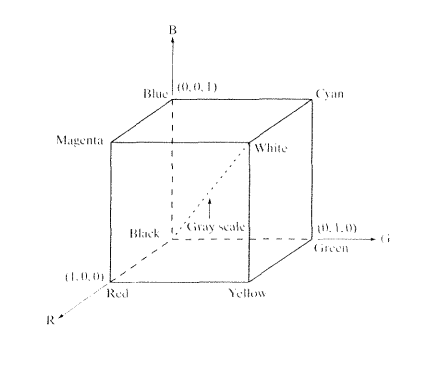
\includegraphics[width=0.80\textwidth]{rgb.png}
\end{center}

In this model, the gray scale (point of equal RGB values) extends from black
to white along the line joining these two point.  The different colors in
this model are point on or inside the cube and are defined by vectors extending
from the origin.

\subsection{The CMY Color Model}
Cyan, magenta and yellow are the secondary colors of light. For instance,
cyan subtracts red light from reflected ``white'' light composed of equal
amounts of red, green and blue light.

Most devices that deposit colored pigments on paper such as color printers
and copies, require CMY data input or perform an RGB to CMY conversion
internally.  Such conversion is performed using the following operation
\[\begin{bmatrix}C\\M\\Y\end{bmatrix}
= \begin{bmatrix}1\\1\\1\end{bmatrix}
- \begin{bmatrix}R\\G\\B\end{bmatrix}\]

\subsection{The HSV Color Model}
Additive colors models such as RGB or CMY as shown above are not well suited
for describing colors in terms that are practical for human interpretation.
When humans view a color object we describe it by its hue, saturation and
brightness.
\begin{center}
  \includegraphics[width=0.69\textwidth]{hsv.png}
\end{center}

While hue is the dominant color as perceived by an observer (red, orange,
or yellow), saturation is the relative purity of color---pure spectrum colors
are fully saturated~\cite{cs5420}.  The definition of value is some what less
trivial, and thus will be shown as Python code converting from BGR to HSV
and vice versa\footnote{This is taken from Python standard library
\texttt{colorsys}, and adapted from RGB to BGR for OpenCV usage.}:
\begin{verbatim}
def bgr_to_hsv(b, g, r):
    """Convert a pixel in BGR to HSV."""
    minc, maxc = min(r, g, b), max(r, g, b)
    if minc == maxc: return 0.0, 0.0, maxc
    diff = maxc - minc
    sat = diff / maxc
    rc, gc, bc = (maxc-r)/diff, (maxc-g)/diff, (maxc-b)/diff
    if r == maxc: return (bc-gc)/6%1, sat, maxc
    if g == maxc: return (2.0+rc-bc)/6%1, sat, maxc
    if b == maxc: return (4.0+gc-rc)/6%1, sat, maxc

def hsv_to_bgr(h, s, v):
    """Convert a pixel in HSV to BGR."""
    if s == 0.0: return v, v, v
    f = h * 6 % 1
    p = v * (1 - s)
    q = v * (1 - s*f)
    t = v * (1 - s*(1 - f))
    i = int(h*6%6)
    if i == 0: return p, t, v
    if i == 1: return p, v, q
    if i == 2: return t, v, p
    if i == 3: return v, q, p
    if i == 4: return v, p, t
    if i == 5: return q, p, v
\end{verbatim}

To use these with images whose pixels stored as 8-bit unsigned integers,
we decorate them with
\begin{verbatim}
def hhu(func):
    return lambda a, b, c: [
        int(i*255) for i in func(a/255, b/255, c/255)]
\end{verbatim}
then the conversion of images stored as NumPy arrays of \verb|uint8|
will be as trivial as
\begin{verbatim}
from itertools import starmap
from numpy import reshape, uint8

def convert_color(image, func):
    x, y, z = image.shape
    return reshape(list(starmap(func, reshape(image, (x*y, z)))),
                   (x, y, z)).astype(uint8)
\end{verbatim}

As a simple test, conversion back and forth should give the same image:
\verb|convert_color(convert_color(image, bgr_to_hsv), hsv_to_bgr)|.
We noticed that our implementation in pure Python is significantly slower
than OpenCV's \verb|cvtColor| which is from a C extension module.


\section{Color Image Enhancements}
\subsection{Contrast Stretching}
Contrast Stretching is a linear image enhancement technique that tries to
improve the contrast by stretching the intensity values of an image to fill the
entire dynamic range.

An image of low contrast has a small difference between its dark and light
pixel values.  The histogram of a low contrast image is usually bends to the
left (mostly light) or to the right (mostly dark), or located around the middle
(mostly gray).  Contrast Stretching computes the highest and the lowest pixel
intensity values, sets them to 255 and 0 respectively, and scales all other
pixel intensities accordingly.
\[\mathrm{contrast} = \frac{I_\mathrm{max}-I_\mathrm{min}}
                           {I_\mathrm{max}+I_\mathrm{min}}\]

\begin{center}
  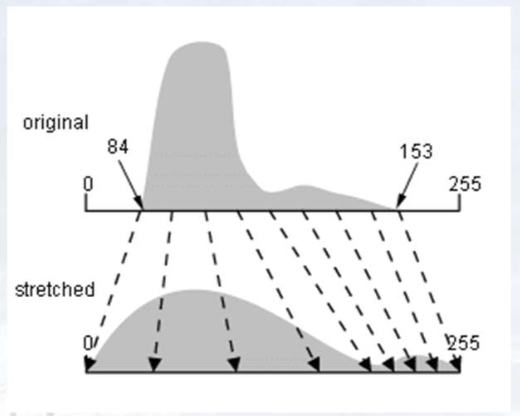
\includegraphics[width = 0.40\textwidth]{contrast-mapping.png}
\end{center}

Both Contrast Stretching or Histogram Equalization can be used to adjust image
intensities to enhance contrast of pictures.  While a non-linear Histogram
Equalization technique is more reliable, in contrast stretching, there exists a
one-to-one relationship of the intensity values between the source image and
the target image i.e, the original image can be restored from the
contrast-stretched image.  This cannot be done with Histogram Equalization.

\subsection{Component Stretching}

\subsection{Local Contrast Enhancement}

\section{Pseudo Color Rendering}
By mapping each intensity level to a color, one may derive a pseudo color image
from a greyscale images.  Typical usage of such technique is in thermal imaging,
elevation and medical imaging to help the human visual system pick out detail,
estimate quantitative values, and notice patterns in data in a more intuitive
fashion~\cite{turbo}.

In OpenCV, this is available under \verb|applyColorMap|.  It is also trival
to reimplement this function only using NumPy:
\begin{verbatim}
import numpy as np

def map_color(grey, mapping):
    r = np.vectorize(lambda i: mapping[i][0])
    g = np.vectorize(lambda i: mapping[i][1])
    b = np.vectorize(lambda i: mapping[i][2])
    # OpenCV uses BGR by default for whatever reason.
    return np.stack((b(grey), g(grey), r(grey)), axis=-1)
\end{verbatim}

For demonstration, we are going to use the Turbo colormap~\cite{turbo}.
We initially considered solely changing the hue based on intensity,
which is also known as the rainbow map, however it is not a visually
intuitive mapping~\cite{rainbowbad}.

Firstly, we tried to apply the mapping on the heightmap of mainland Vietnam and
its neighboring regions\footnote{The original images are taken from
heightmapper: \url{https://tangrams.github.io/heightmapper/}}.  As seen in
the side-by-side comparison, the colormapped image allows the human eyes
to notice more details, especially the high mountains in the north and
the Khorat Plateau (center of the image).
\begin{center}
  \includegraphics[width=0.49\textwidth]{heightmap-grey.png}
  \includegraphics[width=0.49\textwidth]{heightmap-turbo.png}
\end{center}

In addition, we experimented with pseudo lighting, that is, use colormaps
in place of normal greyscale lighting.  The experiment was carried out on
Phong's game Axuy, where colormapping proved to be an enhancement on helping
players detecting shooting range (Axuy is a first person shooter game).
The video where the game is in action is available on
YouTube\footnote{\url{https://www.youtube.com/watch?v=QVGAaoordpk}}.
\begin{center}
  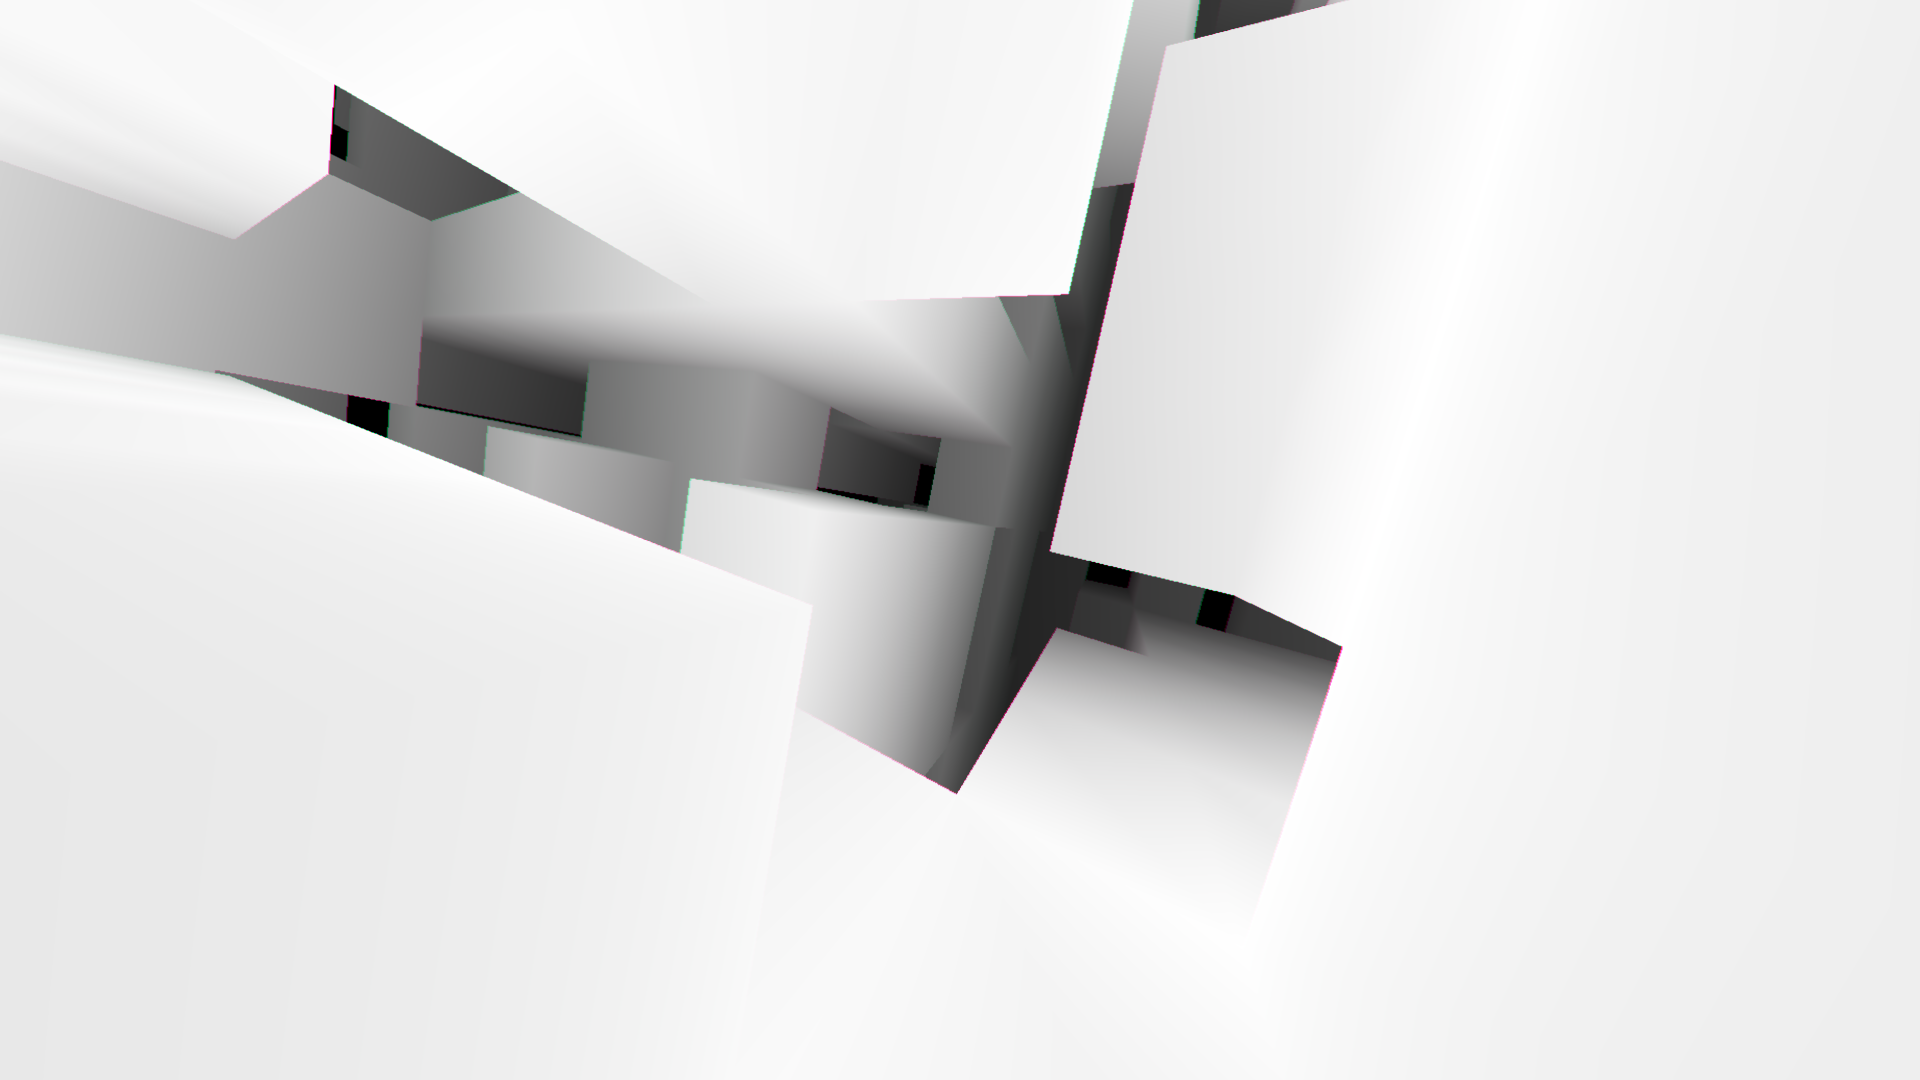
\includegraphics[width=0.49\textwidth]{axuy-grey.png}
  \includegraphics[width=0.49\textwidth]{axuy-turbo.png}
\end{center}

\section{Conclusion}

\begin{thebibliography}{69}
  \bibitem{cs5420} Sanjiv~K.~Bhatia.
    \href{http://www.cs.umsl.edu/~sanjiv/classes/cs5420/lectures/color.pdf}
         {``Color Image Processing''}.
    \emph{CS 5420: Digital Image Processing}.
    University Of Missouri---St.~Louis, Fall 2018.
  \bibitem{rgb} Robert Hirsch.
    \emph{Exploring Colour Photography: A Complete Guide}.
    Laurence King Publishing, 2004. ISBN 1-85669-420-8.
  \bibitem{turbo} Anton Mikhailov.
    \href{https://ai.googleblog.com/2019/08/turbo-improved-rainbow-colormap-for.html}
         {\emph{Turbo, An Improved Rainbow Colormap for Visualization}}.
    Google AI Blog, August 20, 2019.
  \bibitem{rainbowbad} Noeska Smit.
    \href{https://medvis.org/2012/08/21/rainbow-colormaps-what-are-they-good-for-absolutely-nothing/}
         {\emph{Rainbow Colormaps---What are they good for? Absolutely nothing!}}
    medvis.org, August 21, 2012.
\end{thebibliography}
\end{document}
